\chapter{Desarrollo}
Recordemos de la Figura \ref{fig:diagrama_bloques_objetivo} que nuestro sistema está compuesto por 5 bloques. En este capítulo vamos descomponer y analizar cada bloque para su posterior implementación en la simulación.

\section{Análisis}
\subsection*{Codificador y Modulador}
Estos bloques son en realidad bastante simples. Consta de la sumatoria de dos señales sinusoidales. Para la simulación serían dos generadores establecidos en la combinación de frecuencias que corresponden a un determinado digito. Para crear la codificación, basta con ingresar ambas señales a un sumador. Esto luego debe sumarse a una señal constante de 1, con el fin de poder hacer el producto de la señal resultante con la señal portadora. El resultado de esto es la señal ya modulada, como se muestra en la Figura \ref{fig:bloques_cod_mod}.

\begin{figure}[!htb]
  \centering
  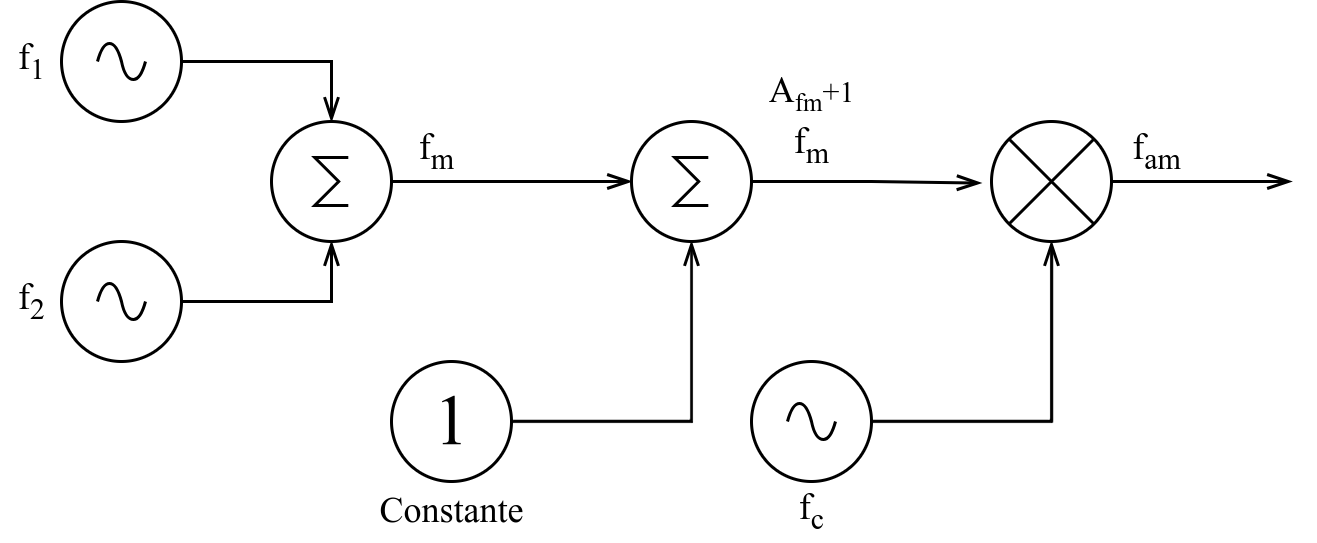
\includegraphics[width=400pt]{images/desarrollo/cod_mod.png}
  \caption{Codificador y Modulador}
  \label{fig:bloques_cod_mod}
\end{figure}

\subsection*{Transmisión}
La transmisión será simulada a través de un filtro pasa-banda, estableciendo las frecuencias de corte de tal forma que el ancho de banda sea el espectro audible por el oído humano, como muestra la Figura \ref{fig:bloques_txs}.

\begin{figure}[!htb]
  \centering
  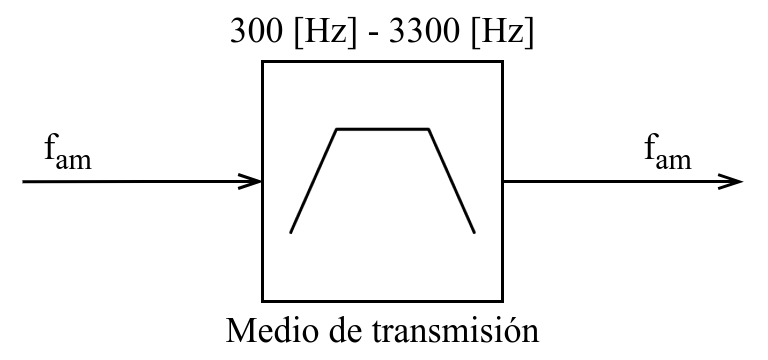
\includegraphics[width=300pt]{images/desarrollo/canal.png}
  \caption{Transmisión}
  \label{fig:bloques_txs}
\end{figure}

\subsection*{Demodulador}
Para demodular la señal, basta con realizar nuevamente el producto con la señal portadora. Como resultado obtenemos la frecuencia moduladora (que es la señal codificada, suma de las frecuencias que componen a un digito específico) como muestra la Figura \ref{fig:bloques_demod}. Luego debemos aplicar un filtro pasa bajos para limpiar la señal de ruidos que puedan haberse introducido, entre esos, algunos vestigios de la señal portadora.

\begin{figure}[!htb]
  \centering
  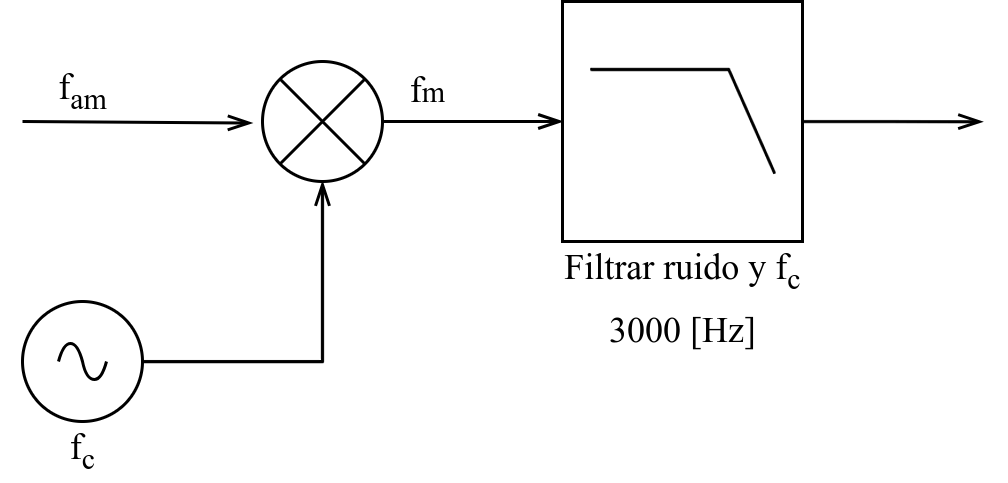
\includegraphics[width=350pt]{images/desarrollo/demod.png}
  \caption{Transmisión}
  \label{fig:bloques_demod}
\end{figure}

\subsection*{Decodificador}
El bloque decodificador es el más complejo de todos, ya que este tiene la lógica para detectar las señales que componen la señal codificada. Como ya vimos en la Figura \ref{fig:diagrama_bloques_decod}, necesitamos 7 filtros pasa-banda para aislar cada una de las frecuencias de la matriz \gls{dtfm}, luego viene la matriz decodificadora. En la Figura \ref{fig:bloques_decod} vemos una simplificación de cómo estaría compuesta esta lógica de decodificación. Cada salida de control es una compuerta AND que se activara cuando sus dos entradas se encuentren activas (o en "1" lógico). Entonces cada compuerta representa la combinación de tonos para detectar cuál fué el digito enviado.

\begin{figure}[!htb]
  \centering
  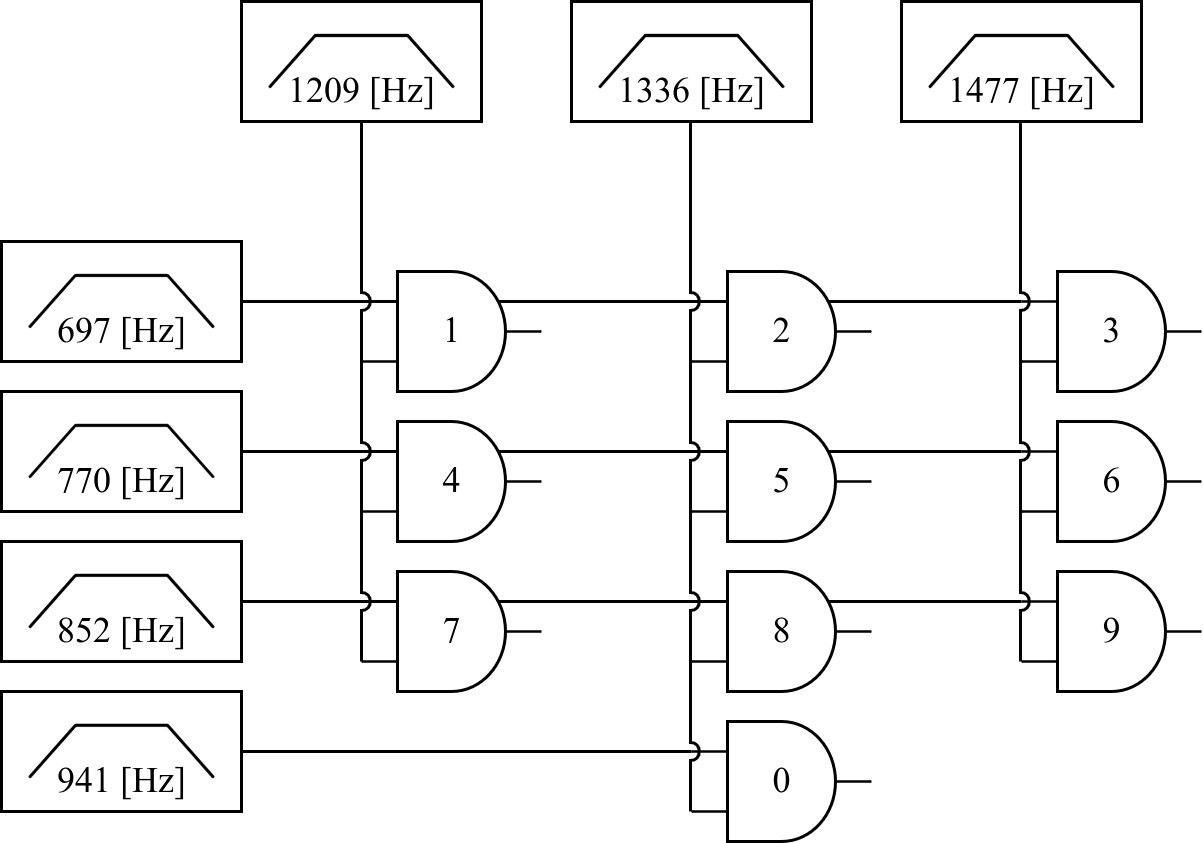
\includegraphics[width=350pt]{images/desarrollo/decod.png}
  \caption{Decodificador}
  \label{fig:bloques_decod}
\end{figure}

\section{Diseño}
Como mencionamos en la sección anterior, para poder implementar los filtros digitales del banco de filtros (bloque decodificador) necesitamos librerías de MATLAB para generarlos, ya que estos filtros serán de alto orden lo que es engorroso para el cálculo analítico. Para hacer uso de estas librerías se crearon 2 \textit{scripts} con el objetivo de automatizar la generación de los filtros en base a parámetros de entrada. En el Código \ref{code:banco_decodificador} podemos ver que se encarga de calcular las frecuecias de corte (inferior y superior) para cada frecuencia central provista, bajo una determinada frecuencia de muestreo y orden específico, esto para el banco de filtros del decodificador. Además de eso, también podemos ver que genera las gráficas para analizar la respuesta en frecuencia de cada filtro, como muestra la Figura \ref{fig:banco_filtros_resp_frec}. Luego en el Código \ref{code:algoritmo_principal} tenemos el algorítmo principal, el cual establece las especificaciones generales del sistema, llama a la función para crear el banco de filtros y además crea el resto de los filtros involucrados como el que representa el canal de transmición y el filtro para eleminar la portadora del espectro de trabajo (en la fase de demodulación).

Se puede notar en el Código \ref{code:algoritmo_principal} que establecemos el orden de los filtros en 6 (para pasa-bajos y/o pasa-altos; se interpreta 12 para pasa-banda). Este valor arbitrario, contrario a los cálculos analíticos del capítulo anterior, es empírico; durante varias pruebas de simulación, los filtros pasa-banda de alto orden (20 aproximadamente) demostraban comportamientos inesperados y no concluyentes a la hora de filtrar señales específicas. Por eso, luego de varias pruebas encontramos que el orden 6 era suficiente para realizar la simulación con resultados favorables y realistas.

Es de suponer que estos filtros diseñados por matlab son estables, sin embargo no dejamos pasar la oportunidad de hacer un análisis de cada uno. Para realizarlo utilizamos una función cuyo código se puede ver en el Apendice \ref{code:script_analisis}. El resultado se puede ver en los siguientes apendices:

\begin{enumerate}
  \item Filtro pasa-banda centrado en 697 [Hz]: Apendice \ref{fig:analisis_697}.
  \item Filtro pasa-banda centrado en 770 [Hz]: Apendice \ref{fig:analisis_770}.
  \item Filtro pasa-banda centrado en 852 [Hz]: Apendice \ref{fig:analisis_852}.
  \item Filtro pasa-banda centrado en 941 [Hz]: Apendice \ref{fig:analisis_941}.
  \item Filtro pasa-banda centrado en 1209 [Hz]: Apendice \ref{fig:analisis_1209}.
  \item Filtro pasa-banda centrado en 1336 [Hz]: Apendice \ref{fig:analisis_1336}.
  \item Filtro pasa-banda centrado en 1477 [Hz]: Apendice \ref{fig:analisis_1477}.
\end{enumerate}

También se pueden ver los Polos y Ceros de cada filtro en el Apendice \ref{sec:pz}.

\begin{figure}[H]
  \lstinputlisting[
    language=Octave,
    caption={Banco Decodificador},
    label={code:banco_decodificador}
  ]{matlab/desarrollo/banco_decodificador.m}
\end{figure}

\begin{figure}[!htb]
  \centering
  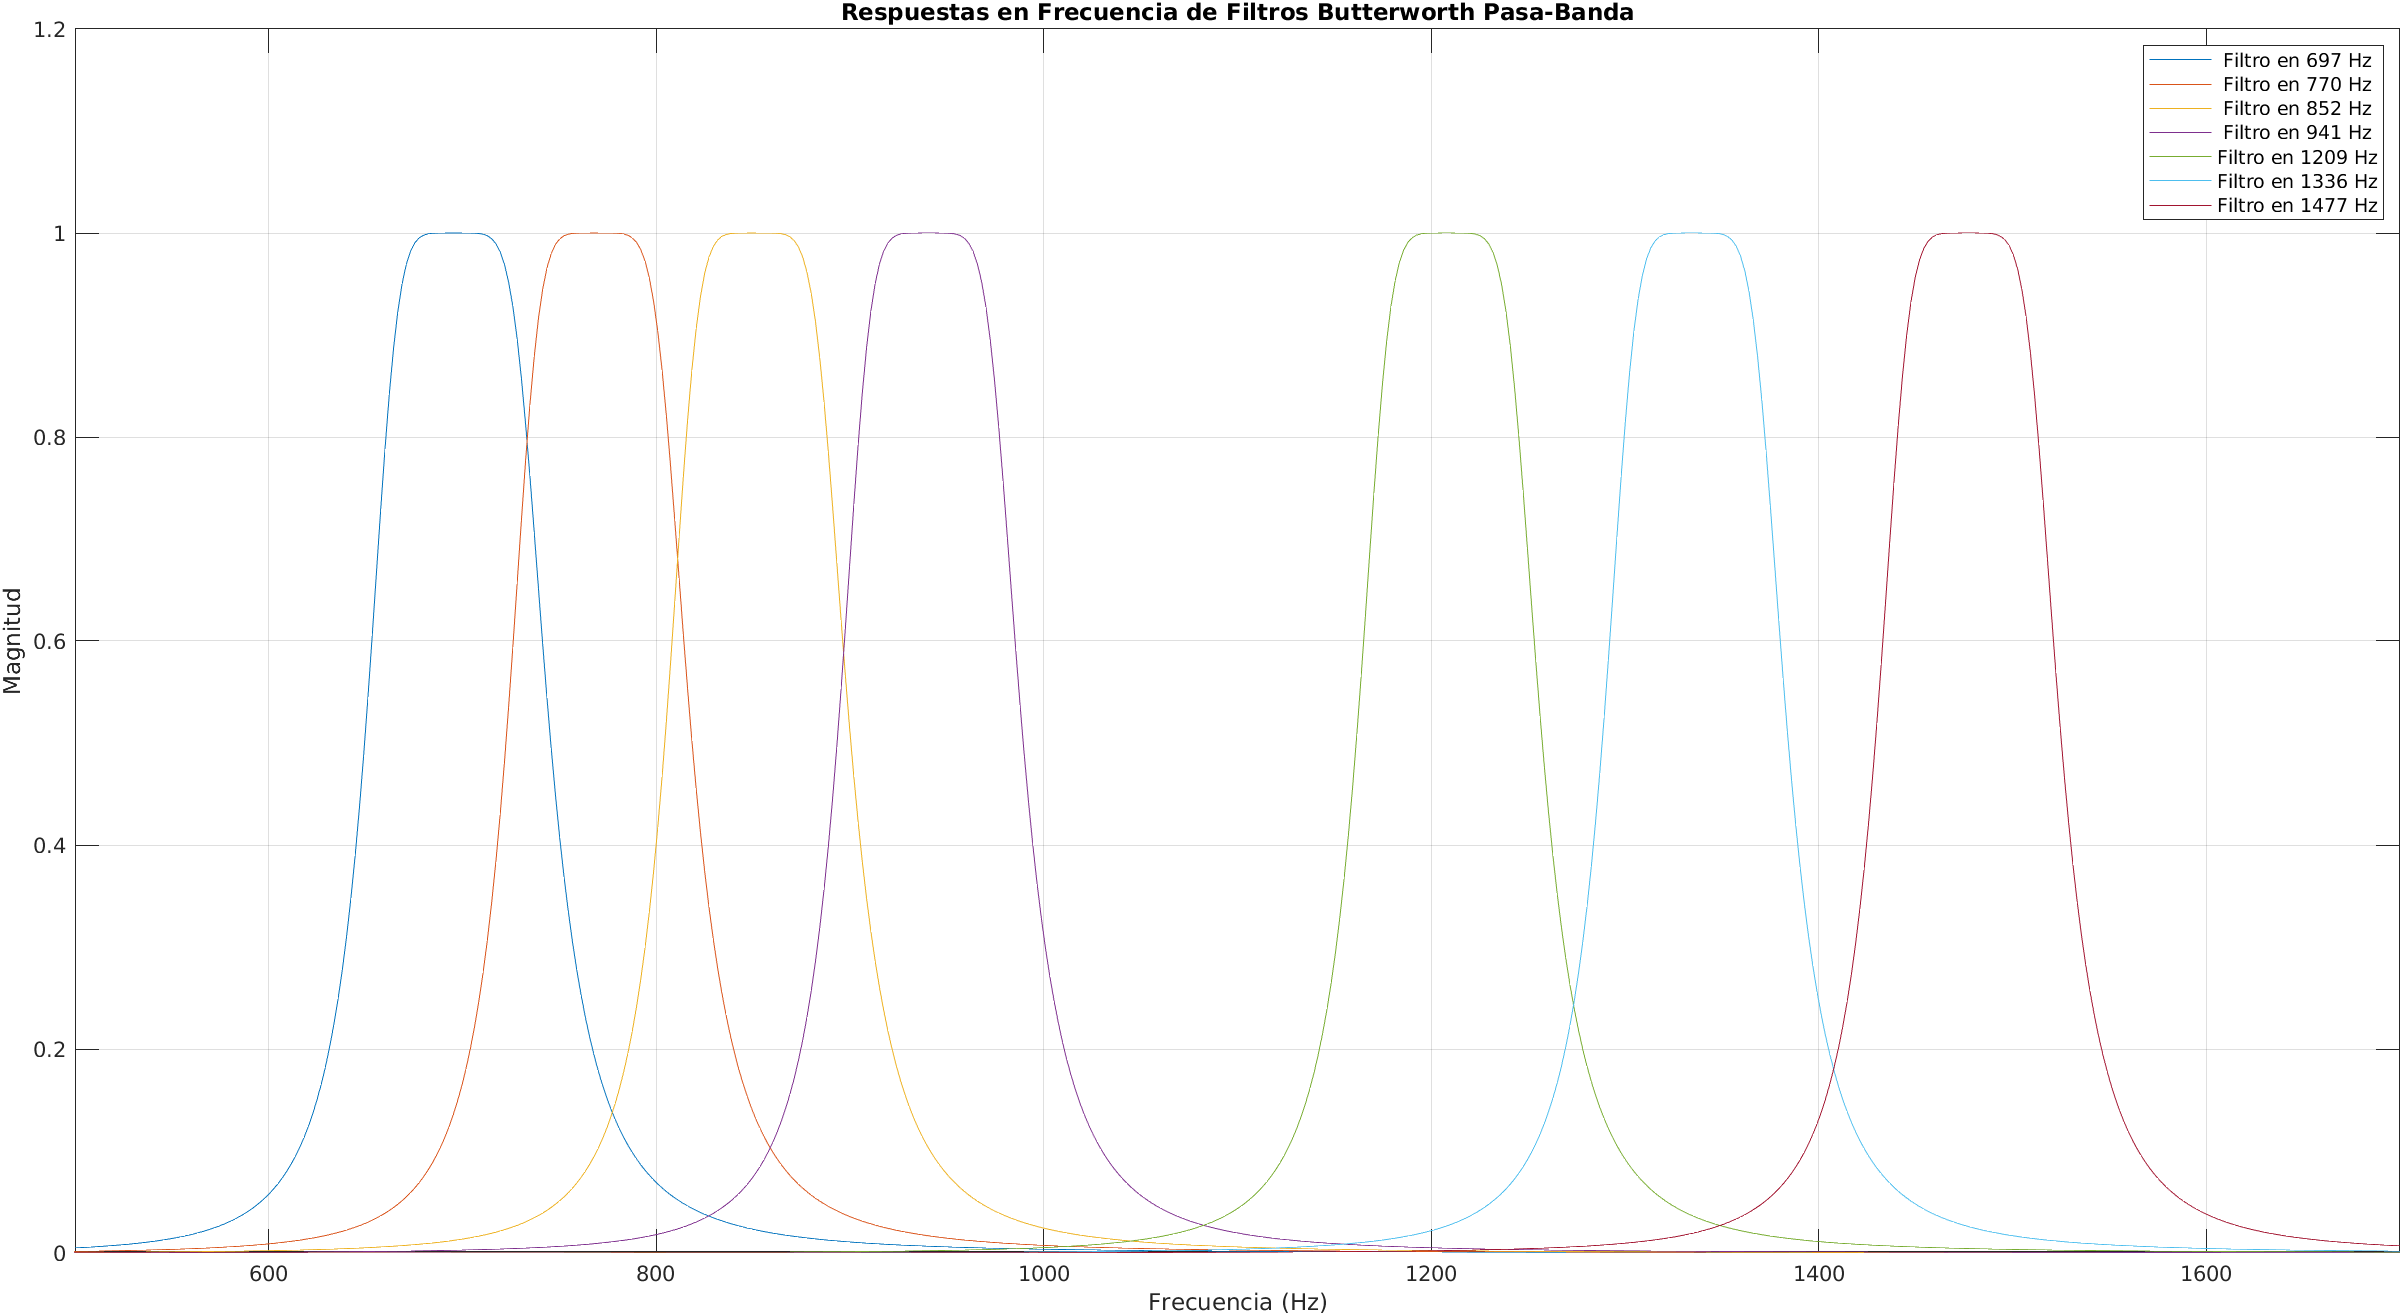
\includegraphics[width=\linewidth]{images/desarrollo/freq_filtros.png}
  \caption{Respuesta en frecuencia del Banco de Filtros}
  \label{fig:banco_filtros_resp_frec}
\end{figure}

\begin{figure}[H]
  \lstinputlisting[
    language=Octave,
    caption={Algorítmo principal},
    label={code:algoritmo_principal}
  ]{matlab/main.m}
\end{figure}

\section{Prototipo}
En base a los resultados obtenidos de los \textit{scripts} diseñamos el sistema completo, en los que cada bloque se alimenta de los datos resultantes. En la Figura \ref{fig:bloques_modem} podemos ver los bloques intervinientes en la primera parte del sistema, esta incluye la selección de los tonos (inferior y superior) para luego sumarlos y lograr la codificación \gls{dtfm} del número 5 en este caso. Luego pasamos a los bloques intervinientes en la modulación AM de las señales, sumando antes una constante 1 para poder realizar el producto con la señal portadora. Una vez obtenida la señal modulada en AM, esta se transmite por el canal de modulación, que según las especificaciones tiene el ancho de banda del espectro audible por el oído humano. Luego llega a la etapa de demodulación, en la que la señal se vuelve a batir (producto) con la portadora, y el resultado es una señal que tiene una componente en la frecuencia de la portadora y debe ser filtrada, por ello utilizamos un filtro pasa-bajos con frecuencia de corte 3[kHz]. Pasado este filtro, la señal obtenida es casi identica a la sumatoria de los dos tonos.

La segunda parte del sistema comprende la decodificación \gls{dtfm} a través de un banco de filtros y una matriz decodificadora, como se muestra en la Figura \ref{fig:bloques_codec}. Primero debemos aislar las señales por tonos diferenciados, esto lo hace el banco de filtros digitales. Cada uno de estos es un filtro pasa-banda con frecuencia central en uno de los 7 tonos, de esta forma logramos aislar cada señal. Dado que estas son sinusoidales, necesitamos calcular el valor efectivo de las mismas para poder operar lógicamente ellas, entonces se coloca un bloque que realiza el cálculo. Luego, el valor obtenido es un número decimal, del cual nos interesa la parte entera, ya que con este dato vamos a validar la amplitud con la que la señal sale del filtro. La razón de hacer este procedimiento es que para poder comparar lógicamente las señales presente para determinar qué tono fue codificado y enviado, lo cual se explica a continuación.

\begin{figure}[!htb]
  \centering
  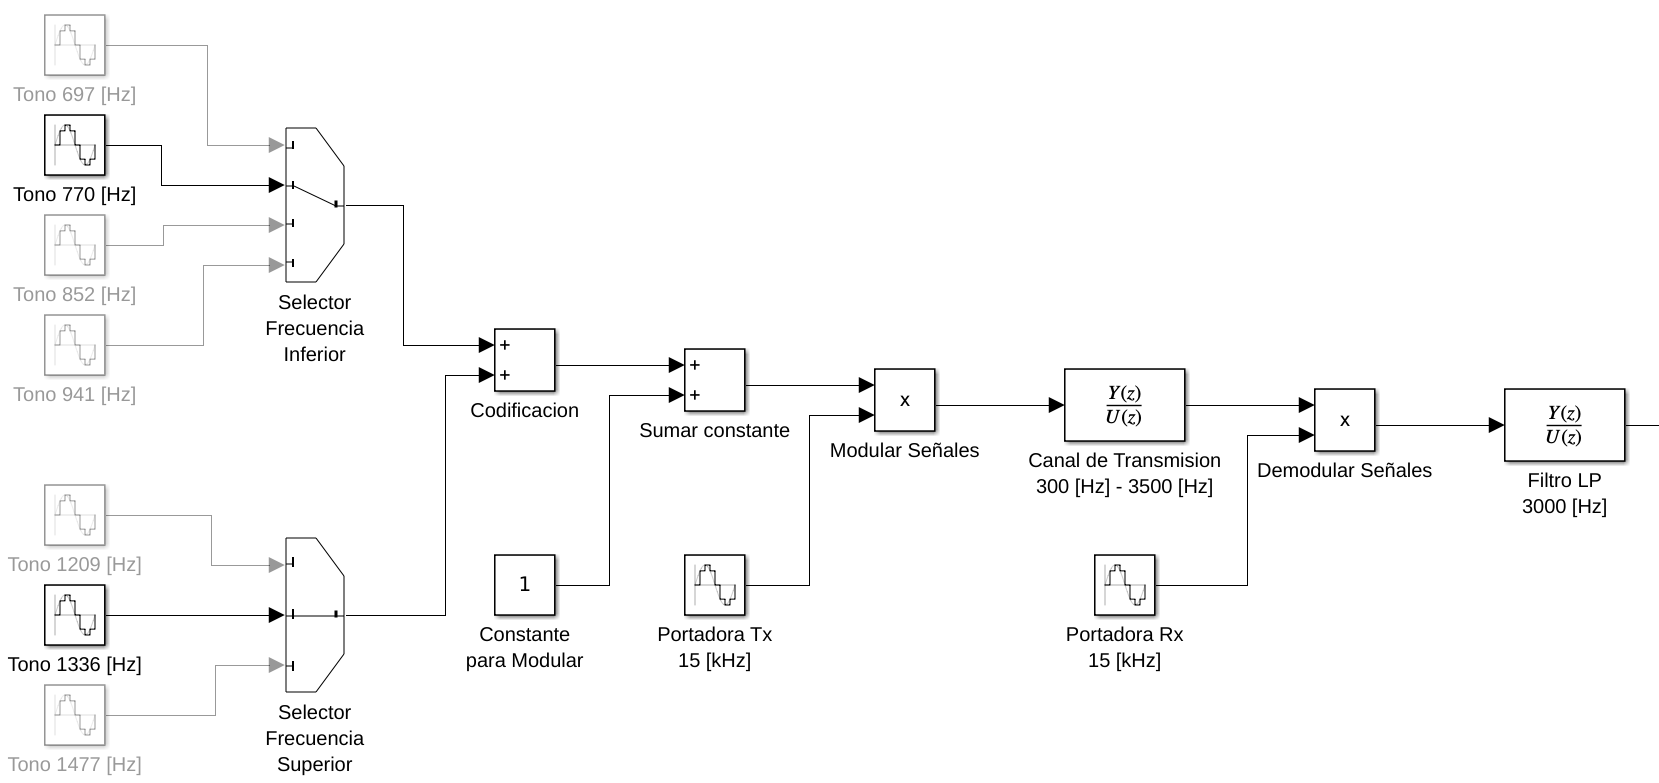
\includegraphics[width=\linewidth]{images/desarrollo/modem.png}
  \caption{Codificación, Modulación, Transmisión y Demodulación}
  \label{fig:bloques_modem}
\end{figure}

\begin{figure}[!htb]
  \centering
  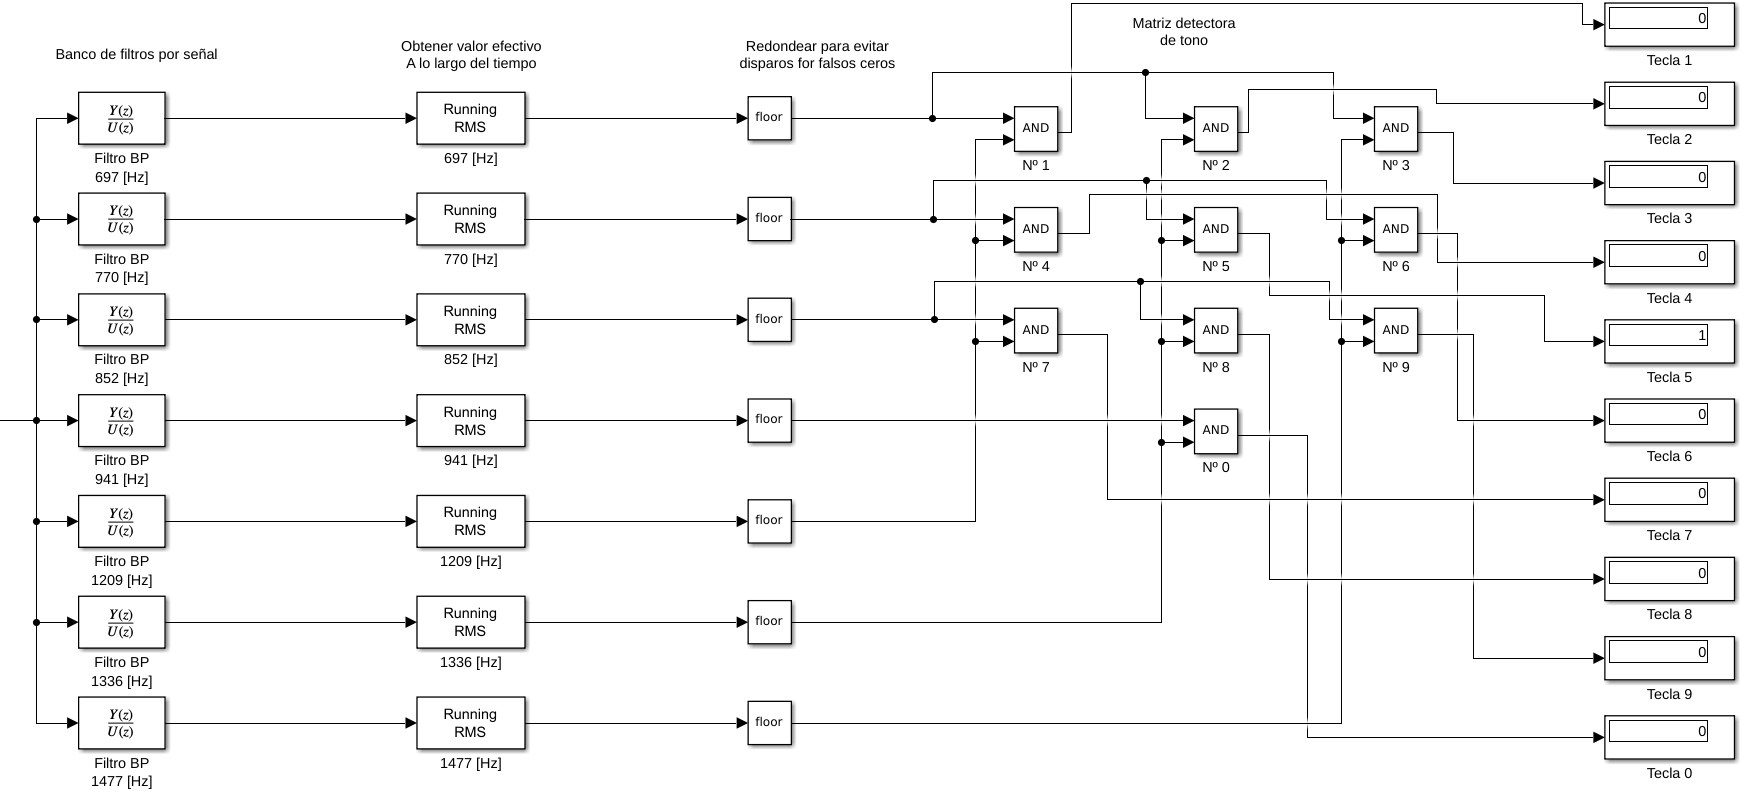
\includegraphics[width=\linewidth]{images/desarrollo/codec.png}
  \caption{Banco de filtros y Decodificador}
  \label{fig:bloques_codec}
\end{figure}

La matriz decodificadora se compone de bloques de operación lógica AND. La salida de este bloque será 1 si y solo si ambas entradas son diferentes a 0\footnote{En el álgebra booleana aplicada en sistemas de control, todo valor igual a 0 se toma como "Falso", mientras que cualquier valor distinto de 0, por más infinitesimal que sea, es "Verdadero"}. Como los filtros anteriores son de orden relativamente bajo, es posible que al tratar las señales dejen pasar vestigios de la otra señal en la codificación pero con mucha menor amplitud. El valor efectivo de este resultado puede ser muy bajo, infinitesimal, del orden de $10^{-2}$, pero no 0 y por consiguiente el operador lógico lo tomará como válido y puede disparar falsos valores. Por esa razón debemos tomar la parte entera del valor eficaz, para garantizar que solo se debe tomar como válida a las señales que realmente son de la misma frecuencia que la frecuencia central de cada filtro.

\section{Simulación}
Para llevar a cabo la simulación vamos a considerar una serie de escenarios posibles, en los que se diferencia mayormente la confiabilidad en el canal de transmisión. Es decir, confiaremos en los bloques de control ya que son implementados a través de sistemas computacionales, pero el medio de transmisión es analógico y su eficacia depende de muchos factores físicos. Este se puede ver alterado de diversas maneras haciendo que parte de la información se pierda o corrompa. Para ello vamos a probar los siguientes escenarios:

\begin{enumerate}
  \item El canal de transmisión es del tipo AWG-24 de menos de 200 [m] de largo, cuyo ancho de banda es de 1 [MHz].
  \item El canal de transimsión es extenso y tiene el ancho de banda del espectro audíble por los humanos.
  \item El mismo canal anterior presenta fallas atenuando en diferentes frecuencias dentro del espectro de tonos \gls{dtfm}
\end{enumerate}

\subsection{Ancho de banda Extendido - 1 [MHz]}
A los efectos prácticos, un canal de 1 [MHz] de ancho de banda bien podría ser considerado un canal ideal, lo que en la simulación equivaldría a no poner un filtro represtantivo del canal de transmisión. Eso significa que toda la señal que sale del modulador llega al demodulador. Sin embargo, realizaremos la simulación utilizando un filtro en el canal para obtener resultados lo más realista posible.

Dado de que la frecuencia de muestreo es de 44 [kHz], y por el Teorema de Nyquist-Shannon, la máxima frecuencia a muestrear debería ser menor o igual a la mitad de la frecuencia de muestreo. Por ello vamos a tomar que el canal tiene un ancho de banda que va desde 0 [Hz] hasta 20000 [Hz]. Este será implementado con un filtro Butterworth de 2do orden pasa-bajos para obtener para obtener una respuesta plana en la banda de paso.

Para realizar esta simmulación, haremos una modificación en el Código \ref{code:algoritmo_principal}, cambiaremos la banda de paso del filtro del canal con los valores \lstinline{butter(2, 22000 / (Fs / 2))}, ejecutamos el \textit{script} y probaremos enviar el número 1.

\begin{figure}[!htb]
  \centering
  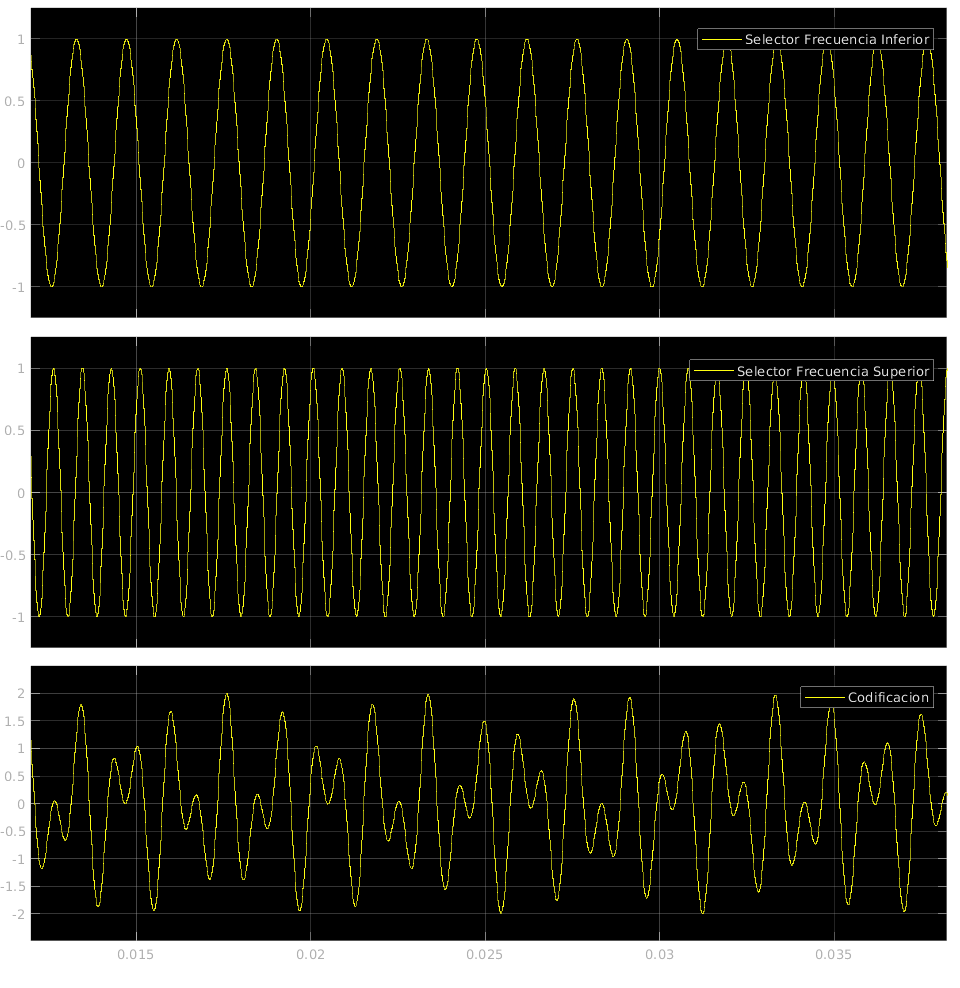
\includegraphics[width=\linewidth]{images/simulacion/extendido/cod.png}
  \caption{Codificación del número 1}
  \label{fig:sim_cod}
\end{figure}

En la Figura \ref{fig:sim_cod} podemos observar la etapa de codificación. Las 2 primeras señales son la frecuencia inferior y superior que componen al número 1 (697 [Hz] y 1209 [Hz]), y la tercera es el resultado de sumar ambas señales.

\begin{figure}[!htb]
  \centering
  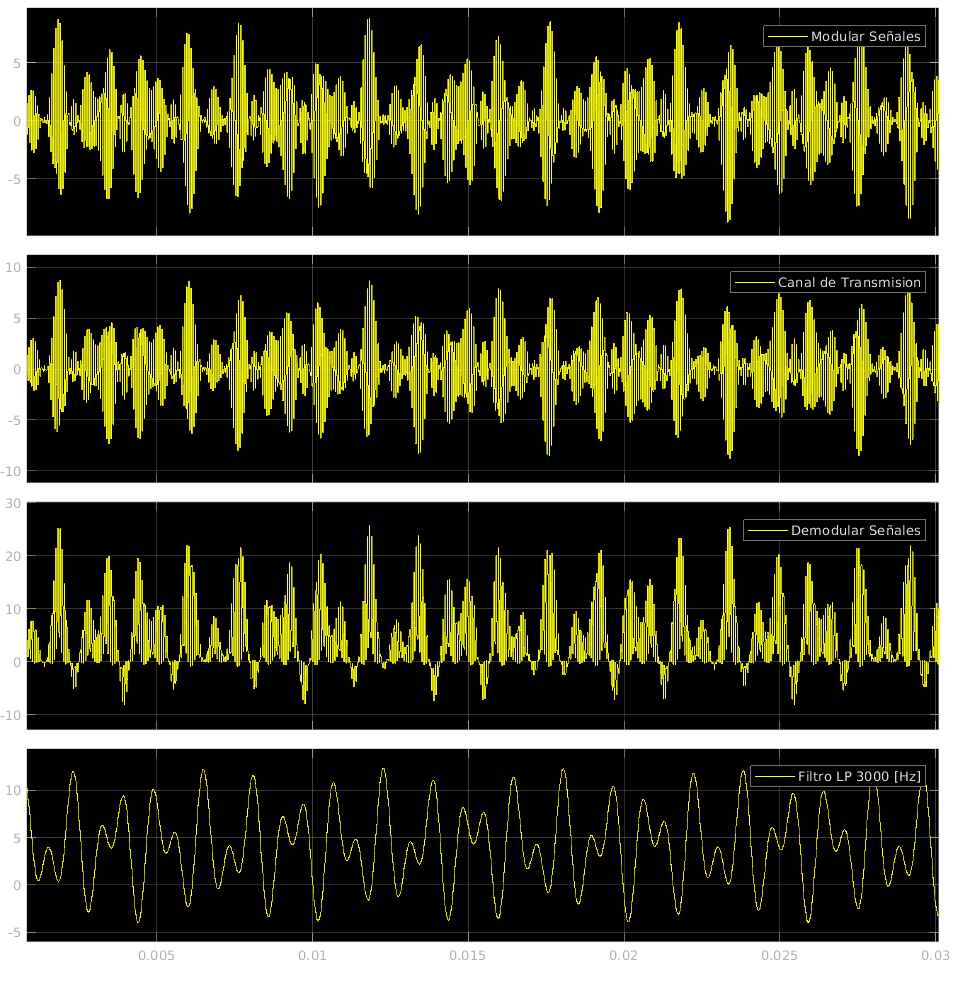
\includegraphics[width=\linewidth]{images/simulacion/extendido/modem.png}
  \caption{Modulación, Transmisión y Demodulación}
  \label{fig:sim_modem}
\end{figure}

En la Figura \ref{fig:sim_modem} tenemos 4 muestras. La primera es la señal modulada, es decir la portadora modulada por la señal codificada del número 1. En la segunda muestra es la misma señal pero a través del filtro represtantivo del canal. Podemos notar que son similares pero se encuentran desfasadas, y esto se debe al filtro en sí. También podemos obervar que la señal no tuvo perdidas de ganancia, mantiene la amplitud con la que salío del modulador. En la tercera muestra vemos la señal luego de ser demodulada, en la que podemos ver que no tiene la forma de la señal codificada, y esto es porque aún tiene una componente de la frecuencia de la señal portadora. En la cuarta muestra vemos que la señal ya tiene la forma de la señal codificada, esto es porque pasó por el filtro pasa-bajos a 3000 [Hz], eliminando así dicha componente.

\begin{figure}[!htb]
  \centering
  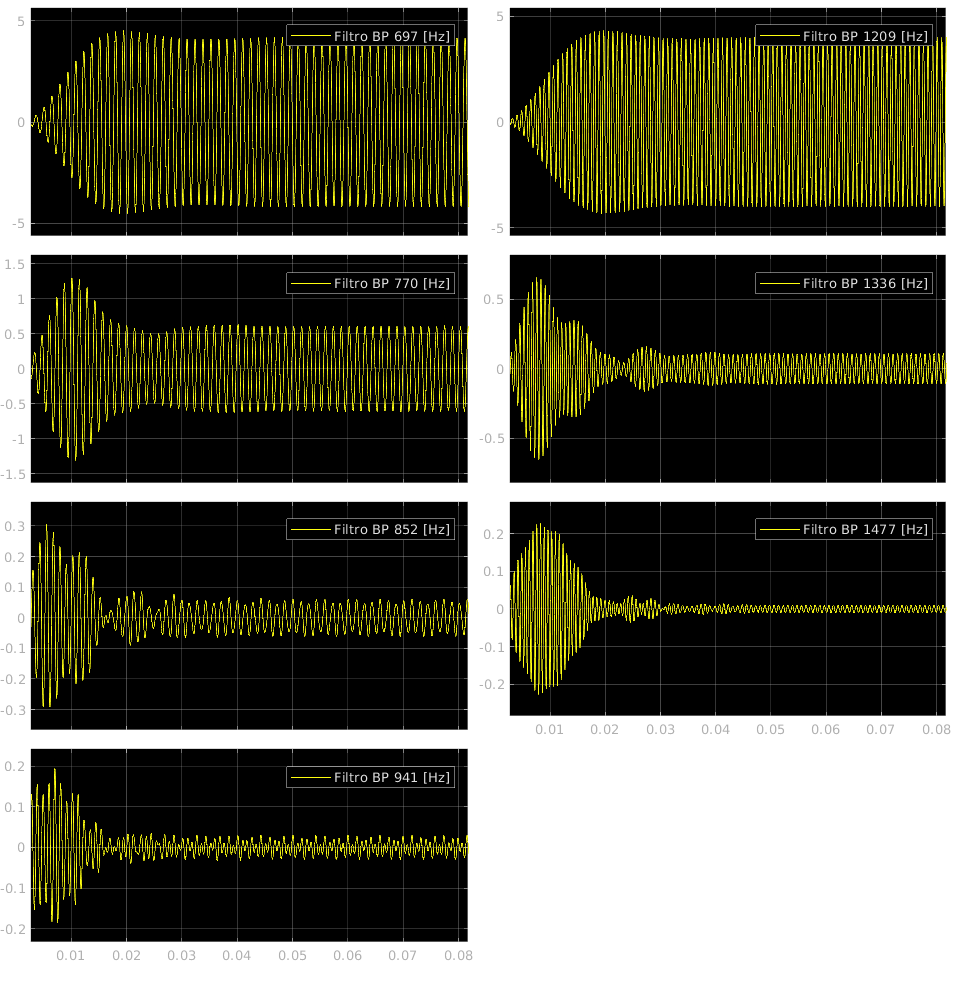
\includegraphics[width=\linewidth]{images/simulacion/extendido/bank.png}
  \caption{Salida del Banco de Filtros}
  \label{fig:sim_bank}
\end{figure}

Una vez tratada y obtenida la señal deseada, puede pasar al banco de filtros para poder aislar las señales que componen la codificación. En la figura \ref{fig:sim_bank} obervamos la respuesta de cada filtro a la señal, y podemos notar rápidamente que en los filtros de 697 [Hz] y 1209 [Hz] las salidas son con mayor intensidad (porque son las que realmente buscamos aislar), mientras que en las otras se atenúa considerablemente. En algunos filtros se atenúa más que otros y esto se debe al solapamiento que tienen los filtros debido a la proximidad de las frecuencias en cuestión.

\begin{figure}[!htb]
  \centering
  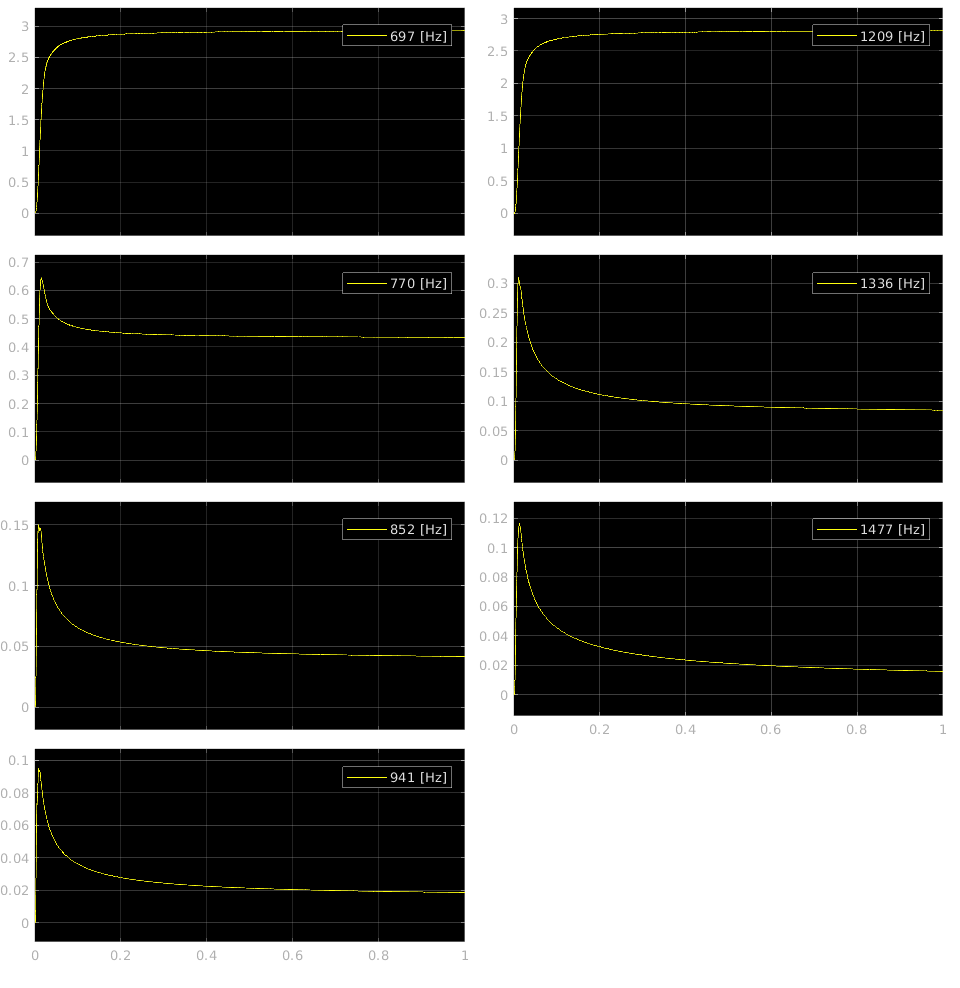
\includegraphics[width=\linewidth]{images/simulacion/extendido/rms.png}
  \caption{Valor Eficaz del Banco de Filtros}
  \label{fig:sim_rms}
\end{figure}

Luego de aislar las señales, necesitamos obtener el valor eficaz de cada salida. En la Figura \ref{fig:sim_rms} obervamos las salidas de cada bloque RMS y claramente de los filtros que no que no son de interés se obtiene valores muy pequeños en contraste con los 2 que sí nos interesa. El paso siguiente es obtener el valor númerico de esas salidas para obtener solamente la componente entera, que en nuestra simulación determina que esa señal está activa.

\begin{figure}[!htb]
  \centering
  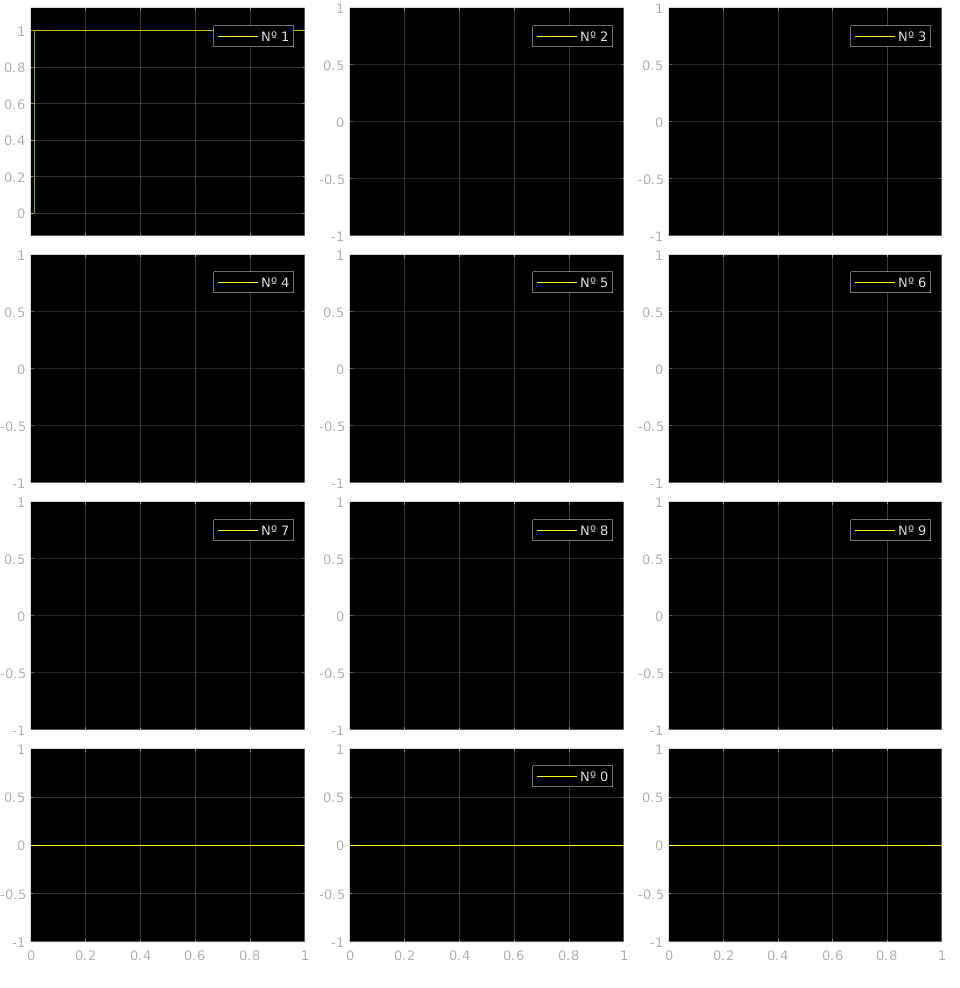
\includegraphics[width=\linewidth]{images/simulacion/extendido/decod.png}
  \caption{Decodificación de las Señales}
  \label{fig:sim_decod}
\end{figure}

Para finalizar obersvamos las salidas de las compuertas lógicas de la matriz decodificadora. En la Figura \ref{fig:sim_decod} tenemos cada muestra dispuesta como un teclado numérico, con su etiqueta correspondiente. Notamos que la muestra del número 1 es la única que tiene valor alto (1 lógico), mientras que las otras están en 0\footnote{En algunas muestras no se logra ver la señal debido a fallas en la renderización de la gráfica, pero si fueran 1 se verían como la primera muetra}. Para mejorar la visualización del funcinamiento, en la Figura \ref{fig:sim_sim} se muestran los Visores al final del sistema, los cuales muestran los valores de las señales de la matriz decodificadora, y nuevamente, vemos que todas están en 0 con la excepción de la tecla número 1.

\begin{figure}[!htb]
  \centering
  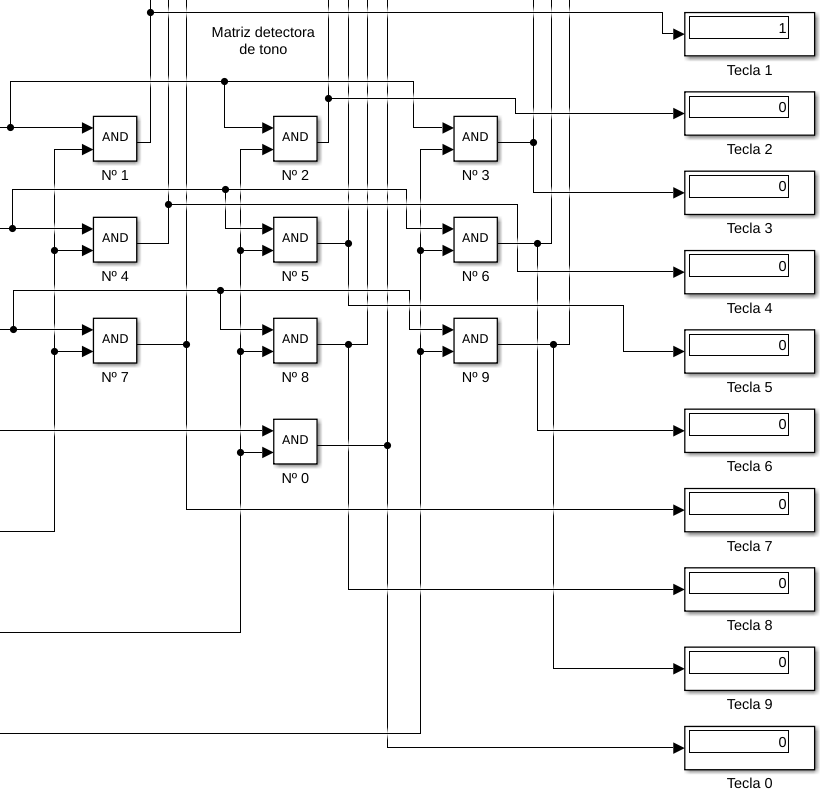
\includegraphics[width=400pt]{images/simulacion/extendido/sim.png}
  \caption{Visor de la Simulación}
  \label{fig:sim_sim}
\end{figure}


\subsection{Ancho de banda Reducido - 3 [kHz]}
Para esta simulación, modificamos nuevamente el Código \ref{code:algoritmo_principal} para que vuelva a operar con el canal real, establecido entre 300 [Hz] y 3500 [Hz]. Por motivos de simplicidad la simulación la vamos a analizar directamente desde el canal, ya que la etapa de codificación no se modifica.

Para empezar, vamos a hacer un análisis de la estabilidad del canal ya que este ahora es diferente al canal "ideal" del apartado anterior. Para ello hicimos uso del Código \ref{code:script_analisis} y obtuvimos los resultados que se muestran en la Figura \ref{fig:real_chan}. Se puede observar que los polos indican que el filtro es estable, sumado a que la respuesta al impulso y al escalón también lo reafirman. Pero lo que llama la atención aquí es la respuesta en frecuencia del filtro. Es de esperarse que la curva tenga esa forma, ya que para eso fue diseñado, pero vemos también que está filtrando componentes de alta frecuencia, casualmente entre ellas se encuentra la señal portadora. Vamos a analizar si esto representa un problema para la simulación.

\begin{figure}[!htb]
  \centering
  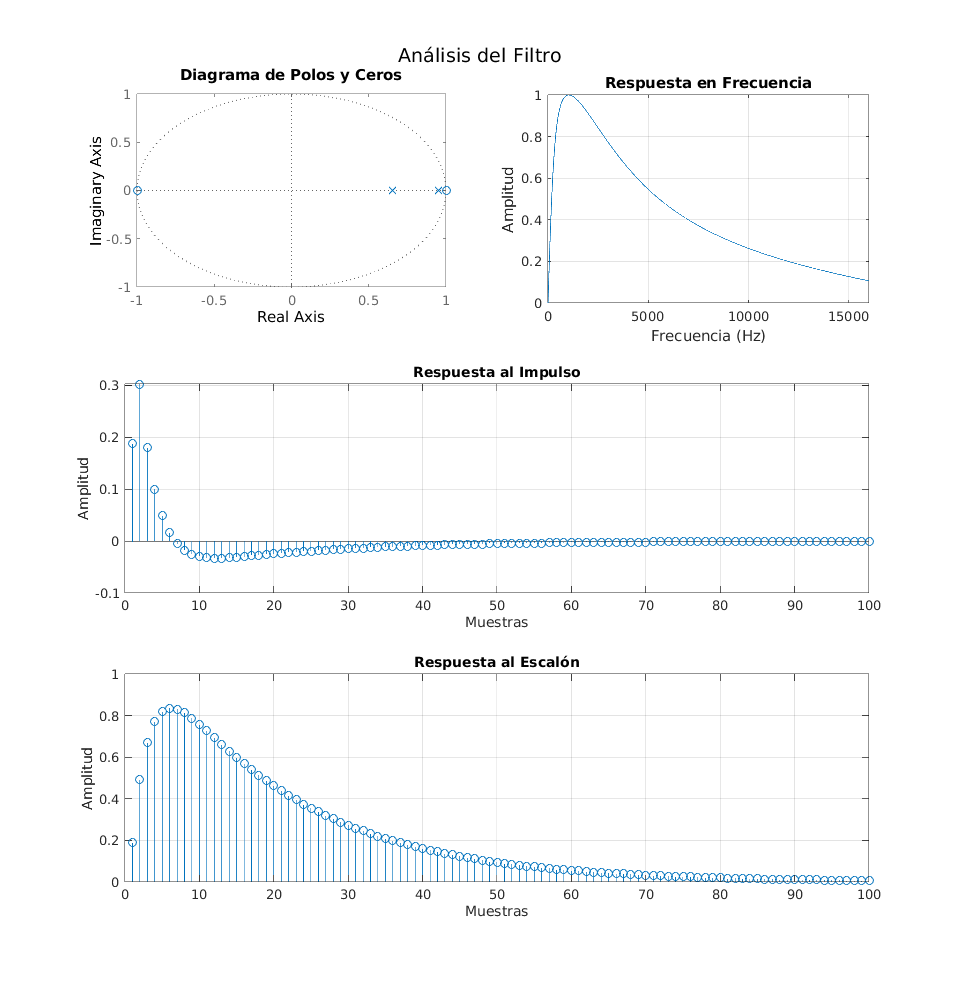
\includegraphics[width=\linewidth]{images/simulacion/reducido/chan.png}
  \caption{Estabilidad del Canal}
  \label{fig:real_chan}
\end{figure}



\begin{figure}[!htb]
  \centering
  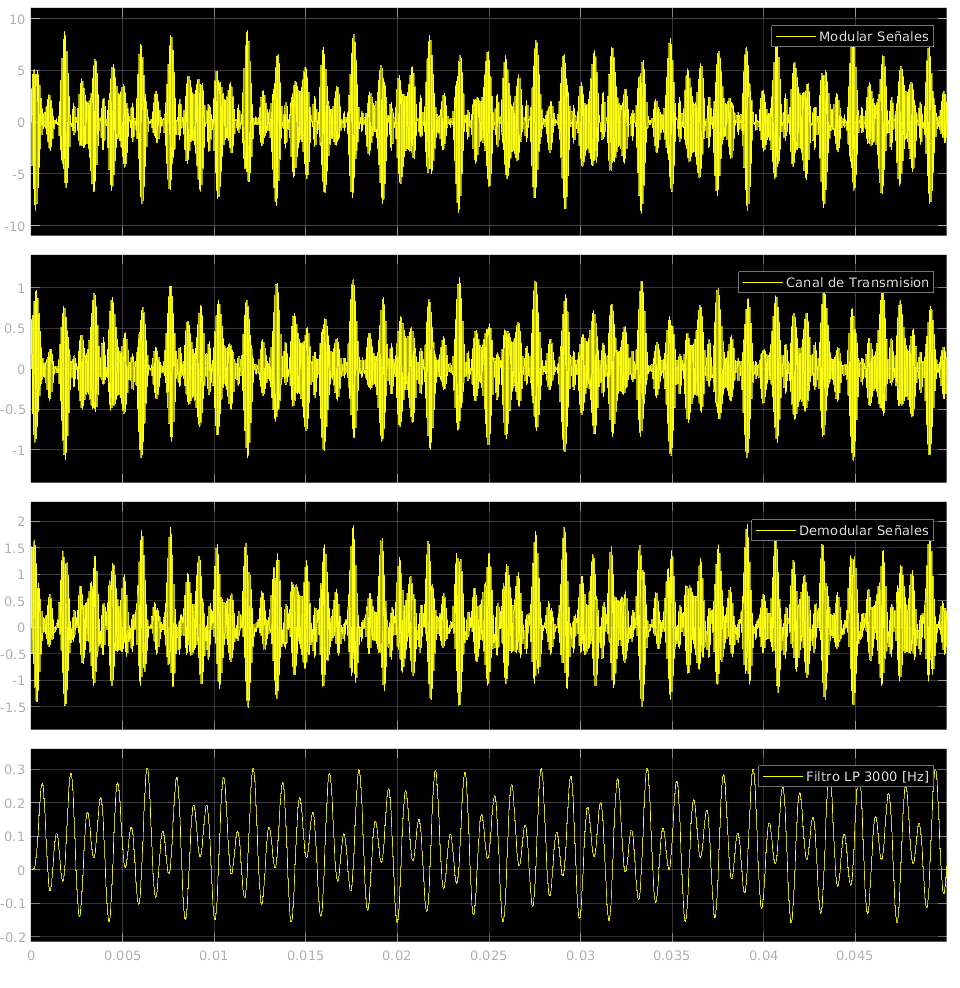
\includegraphics[width=\linewidth]{images/simulacion/reducido/modem.png}
  \caption{Modulación, Transmisión y Demodulación}
  \label{fig:real_modem}
\end{figure}

\pagebreak

En la Figura \ref{fig:real_modem} vemos que al pasar por el canal, la señal se ve drásticamente atenuada (casi 10 veces menos) lo cual ya puede significar un problema considerando que en el ejemplo anterior esto no pasaba. Luego de pasar por el demodulador, la señal parece que no sufrió ningún cambio, esto pude ocurrir porque la componente con mayor amplitud (la portadora) ha sido filtrada, con lo cual la demodulación ya no tiene sentido. Y luego pasando por el filtro que estaba destinado a filtrar la portadora, la señal pierde más ganancia. Todo parece indicar que el sistema no va a funcionar correctamente debido a que la señal llega con poca fuerza al banco de filtros.

\begin{figure}[!htb]
  \centering
  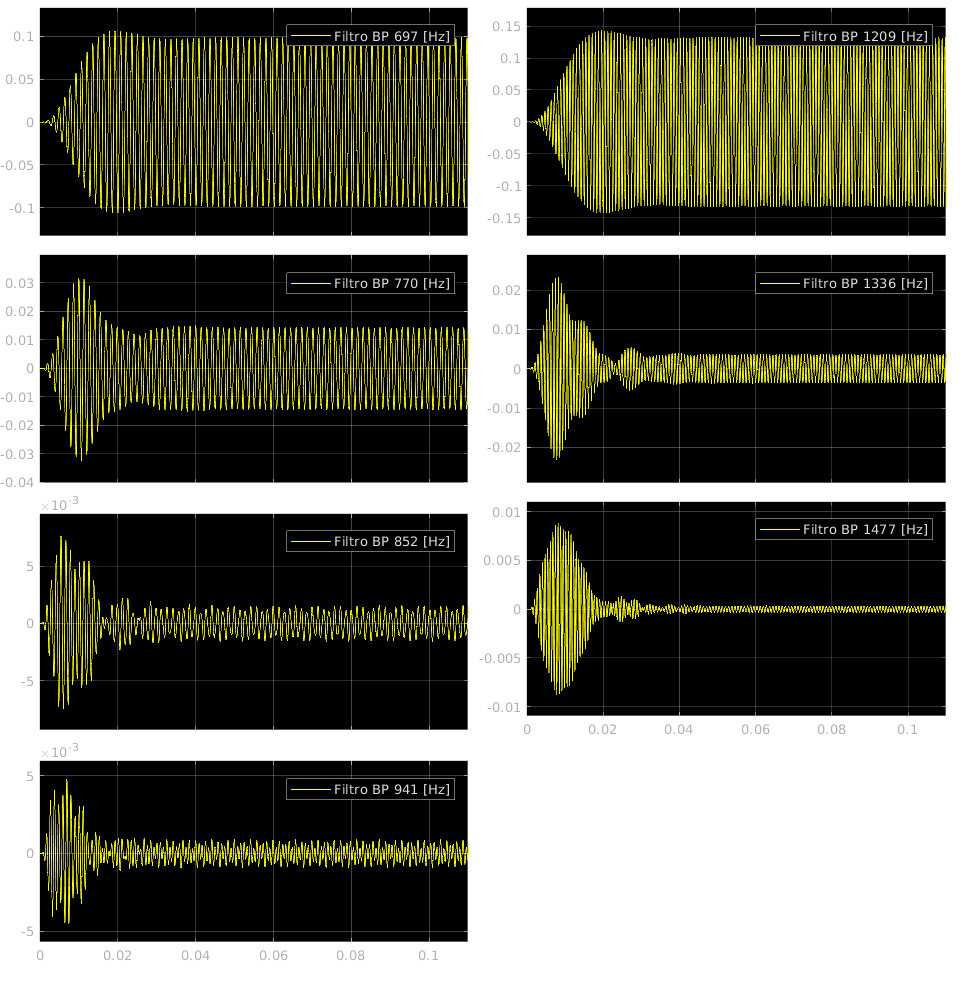
\includegraphics[width=\linewidth]{images/simulacion/reducido/bank.png}
  \caption{Salida del Banco de Filtros}
  \label{fig:real_bank}
\end{figure}

\begin{figure}[!htb]
  \centering
  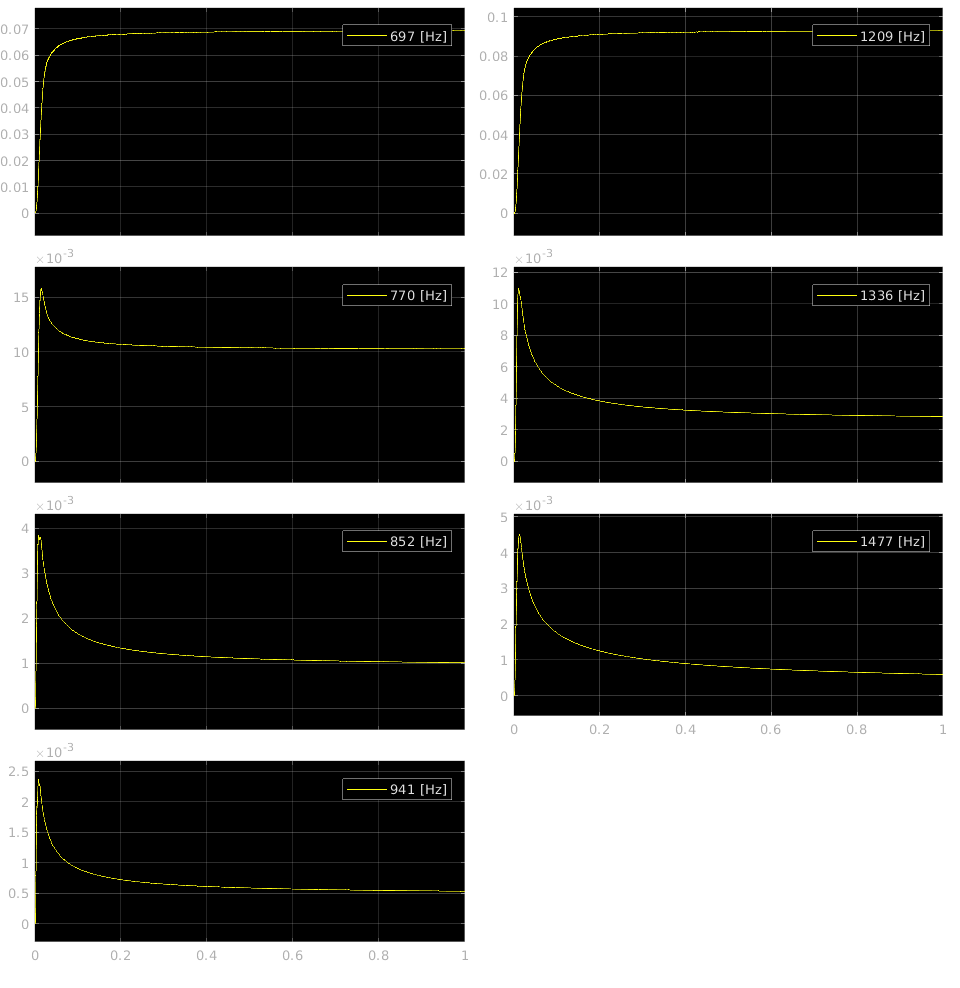
\includegraphics[width=\linewidth]{images/simulacion/reducido/rms.png}
  \caption{Valor Eficaz del Banco de Filtros}
  \label{fig:real_rms}
\end{figure}

\pagebreak

Al pasar por el banco de filtros, como muestra la Figura \ref{fig:real_bank}, podemos notar que las señales son correctamente aisladas. Es decir que la señal codificada se puede detectar, pero estas tiene muy poca amplitud. Por consiguiente, el valor eficaz será aún menor y numericamente ninguna señal no conseguirá pasar la unidad (en magnitud), como se puede ver en la Figura \ref{fig:real_rms}.

\begin{figure}[!htb]
  \centering
  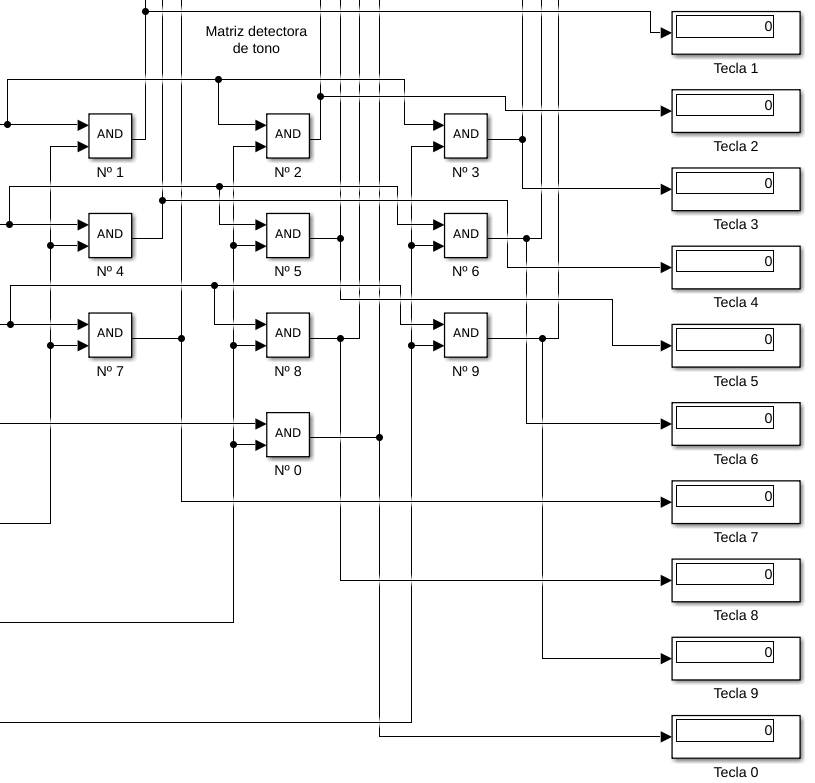
\includegraphics[width=400pt]{images/simulacion/reducido/sim.png}
  \caption{Visor de la Simulación}
  \label{fig:real_sim}
\end{figure}

\pagebreak

En consecuencia, podemos ver en el visor del sistema (Figura \ref{fig:real_sim}) que ninguna tecla se encuentra activa, ya que las señales no tienen una amplitud adecuada para lograr activar las compuertas.

Esto lo podemos analizar desde 2 puntos de vista: el sistema está mal calibrado en cuestiones de umbrales y solo necesita un ajuste (ya que las señales llegan correctamente); o bien, necesitamos aumentar la ganancia de la señal modulada enviada al canal para que el sistema siga funcionando acordementet. Empiricamente, encontramos que aumentar 20 veces la señal a la salida del modulador es suficiente para matener el sistema funcionando correctamente.

\pagebreak

Sin embargo, esto puede ser ineficiente. Claramente el canal de transimsión filtra la señal portadora entonces ¿Es realmente necesaria la modulación? Los sistemas \gls{am} están pensados para medios de transimsión en los que se pueden enviar frecuencias altas (como el aire). En un cable que tiene el ancho de banda de la voz (cable telefónico, por ejemplo) es innecesario el uso de la modulación en amplitud porque la portadora se pierde. Para este mismo sistema bastará envar la señal codificada pero con una amplitud lo suficientemente grande para que pueda a travesar el medio y pueda ser tratada a través del banco de filtros y las demás etapas.

\subsection{Canal con Fallas}